\chapter{Event Reconstruction}
\label{cap4}

\textit{In the search of high mass resonances in the $W^+W^-$ channel, leptons (specifically, electrons or muons), jets and MET are used  to select signal events.
The reconstruction of such objects follow standard algorithms and procedure which have been
developed by the experiment. In this chapter the reconstruction  and the identification algorithms for these objects are described. 
In particular I have contributed in the evaluation of the best b-tagging working points, Tab.~\ref{btt}.}

\section{The Particle Flow}
\label{PFt}
The algorithm for the event reconstruction is called Particle Flow (PF)~\cite{CMS-PAS-PFT-09-001}. Its goal is to reconstruct all stable particles that emerge from a hadron-hadron collision, such as muons, electrons, photons, charged hadrons, and neutral hadrons. The PF technique uses all the information coming from the 
CMS sub-detectors and combines them to obtain: type of particle, direction, momentum, and energy.
The reconstruction of charged particles is done from the hits in the silicon tracker. 
%that is immersed in a uniform magnetic field of 3.8 T. 
Transverse momentum is precisely measured down to about 150 MeV.
The photon and electron reconstruction is performed using the high resolution and high granularity of ECAL together with the excellent tracking system. 
This combination provides a very good energy resolution for electrons. Muons are reconstructed in the muon chambers together with the tracking system.
The reconstruction of charged-particles in the tracker, energy clusters in the calorimeters and muons in the muon chambers are the first steps of the PF. The informations are then connected to each others, making blocks of elements which are topologically compatible.
Starting by blocks, the candidate particles (PF Candidates) are fully reconstructed and identified as:
\begin{itemize}
\item Muons: the combination of a track in the tracker and a track in the muon system gives rise to a PF muon. The corresponding track is removed from the block after the identification.
\item Electrons: a charged-particle track is linked to one or more ECAL clusters (if presents)
\item Charged hadrons: PF charged hadrons are obtained from the remaining tracks. Tracks 
are linked to ECAL and HCAL clusters, and the deposited energy is determined taking into
account the momentum of the track.
\item Photons and Neutral hadrons: PF photons are given by ECAL clusters not compatible with charged-tracks; PF
neutral hadrons instead are given by unaccounted HCAL deposits.
\end{itemize}
After that, once the list of PF Candidates is defined, the PF jets are reconstructed using a clustering algorithm. At the LHC,  at each bunch crossing there are of the order of 20 minimum bias proton-proton interactions, which pollute any interesting hard events with many soft particles. 
The identification and energy measurements for jets will be adversely affected by pileup (PU), with resolution and absolute energy measurements suffering significantly. 
Therefore effects of PU needs to be taken into account and corrected for. At the end the PF MET is evaluated as the opposite of the transverse momentum-vector sum over all reconstructed PF Candidates.\\
In the following, each step of the reconstruction is described in details. 

\section{Tracking}
\subsection*{Hit reconstruction in the pixel and strip detector}
The first step of the reconstruction process is referred to as local reconstruction~\cite{Chatrchyan:2014fea}.  It consists of the clustering of zero-suppressed
signals above specified thresholds in pixel and strip channels into hits,  and then estimating the cluster positions and their uncertainties defined in a local
orthogonal  coordinate  system ($u$, $v$) in  the  plane  of  each  sensor (pixel and strip). 
The  hit reconstruction in the pixel detector and in the the strip detector is described below:
\begin{itemize} 
\item The pixel detector: in the data acquisition system of the pixel detector, zero-suppression is performed in the
readout chips of the sensors, with adjustable thresholds for each pixel.  This pixel readout threshold 
is set to a single-pixel threshold corresponding to an equivalent charge of 3200
electrons.  Offline, pixel clusters are formed from adjacent pixels, including both side-by-side
and corner-by-corner adjacent cells.  Each cluster must have a minimum charge equivalent to
4000 electrons.
\item The strip detector:  the clusters are seeded by any channel passing zero-suppression that has a charge at least a
factor of three greater than the corresponding channel noise. Neighbouring strips are added
to each seed, if their strip charge is more than twice the strip noise. 
A cluster is kept if its total charge is a factor five larger than the cluster noise.
The position of the hit corresponding to each cluster is determined from the charge-weighted
average of its strip positions, corrected for the  Lorentz drift.
\end{itemize}

\subsection*{Track reconstruction}
Different algorithms are used in CMS for track reconstruction,~\cite{Chatrchyan:2014fea, Adam:2005cg}.
All   methods   use   the   reconstructed positions (hits) of the passage of charged
particles inside the CMS silicon detectors to determine the
trajectories of the charged tracks and therefore measure their directions and momenta.  
The Combinatorial Track Finder (CTF) is the main standard algorithm and proceeds in three steps:
\begin{itemize} 
\item Seeding:  pairs or triplets of hits, that are compatible with a charged particle, originated from the interaction region and with $p_T$ above a lower
threshold, are considered as possible candidates of
charged tracks.  Pixel hits provide the best track
seeding, given their three-dimensional position information and lower occupancy.  
\item Finding: is based on a standard Kalman  Filter  pattern  recognition  approach.
The  track trajectory  is  extrapolated  to  the  neighboring tracker  layers, starting from the seeded parameters.
Compatible  hits  are  assigned to the track. 
The Kalman Filter, a  succession of  alternating  prediction  and  filtering  steps, 
updates the track parameters at each steps with new hits.
 The updated tracks are assigned a quality and only the best ones are kept for further propagation. 
\item Fitting: the  final  estimate  of  the   parameters  of
each  track  helix  is  completed  in  the  last  steps
applying again the Kalman Filter for the trajectory fitting.  Each trajectory is refitted using a
least-squares fit. In the central region, $|\eta|<1$, the $p_T$ resolution is better than 1\%  for tracks with $p_T<10\%$. 
At higher $p_T$, the resolution gets worse  as $\Delta (1/p_T) \sim 0.2$ TeV$^{-1}$  approximately.
\end{itemize}
The  reconstruction  of  single  muons  with  the
CTF  algorithm  is  almost  fully  efficient  over  the whole acceptance range.
Electrons, being charged particles, can be reconstructed through the standard track reconstruction.  However,  as electrons lose energy primarily through bremsstrahlung,  rather than ionization,  large energy losses are common.  
The energy loss distribution is highly non-Gaussian, and therefore the standard Kalman filter is not appropriate:
a modified version of the Kalman filter, called the Gaussian Sum Filter (GSF) is used. 
Electron candidates are reconstructed using the  information from the tracker but also from
the ECAL, Sec~\ref{ler}. 
For charged hadrons, finally, there are inefficiencies in the reconstruction due to their nuclear
interactions  in  the  tracker  material. 


\subsection*{Primary-vertex reconstruction}
The goal of primary-vertex (PV) reconstruction~\cite{Speer:927395}  is to measure the location, and the associated
uncertainty, of all proton-proton interaction vertices in each event, including the ``signal'' vertex
and any vertices from pileup collisions, using the available reconstructed tracks.  
It consists of three steps: 
\begin{itemize} 
\item  selection of the tracks;
\item clustering of the tracks that appear to originate from the same interaction vertex;
\item fitting for the position of each vertex using its associated tracks.
\end{itemize}
Track selection involves choosing tracks consistent with being produced promptly in the primary interaction region, by imposing requirements on the maximum value of significance of the transverse impact parameter,  the number of strip and pixel hits associated with a track and the normalized
$\chi^2$ from the fit to the trajectory  ~\cite{Chatrchyan:2014fea}.
The selected tracks are then clustered on the basis of their z-coordinates at their point of closest approach to the centre of the beam spot  using a
\textit{deterministic annealing} (DA) algorithm~\cite{726788}. 
%The algorithm proceeds in a way that is analogous to that of a physical system approaching a state of minimal energy through a series of
%gradual  temperature  reductions. 
%The z-coordinates  of  the  points  of  closest  approach  of  the tracks to the centre of the beam spot are $z_i^T \pm \sigma_i^Z$.
% The tracks must be assigned to some unknown number of vertices at positions $z_k^V$.
%The tracks can be associated with more than one vertex, with probability $p_{i,k}$ that is  the probability of the
%assignment of track $i$ to vertex $k$ in a large ensemble of possible assignments.
% The most probable vertex positions at ``temperature'' T (like in the calculations in statistical mechanics) is,
%\begin{equation}
%F=-T \sum_{i}^{\# \; tracks} p_i \, \log \sum_{k}^{\# \, vertices} \rho_k  \exp [-\frac{1}{T} \frac{(z_i^T-z_k^V)^2}{(\sigma_i^z)^2}  ]
%\end{equation}
% relative to the positions of the vertices $z_k^V$ with vertex weights $\rho_k$ (the weights are variable, but the sum is always constrained
%to unity).
%The DA algorithm is initiated at a very high temperature with a single vertex and $T$ is gradually decreased.
%This procedure tracks the global minimum of $F$ from high to low temperature.
%The number of vertices increases as the temperature falls, and rises each time the minimum of $F$ turns into a saddle point at lower temperatures. 
The DA process finds not only positions and assignments of tracks to vertices but also the  number of vertices.
In Fig.~\ref{Fig:pu} is shown the distribution of the number of vertices in a Drell-Yan sample. This distribution is related to the number of PU events. Therefore MC events are re-weighted according to the ratio between data and simulation in the number of primary vertices in order to correct for the different pileup. 
\begin{figure*}[htbp]
\centering
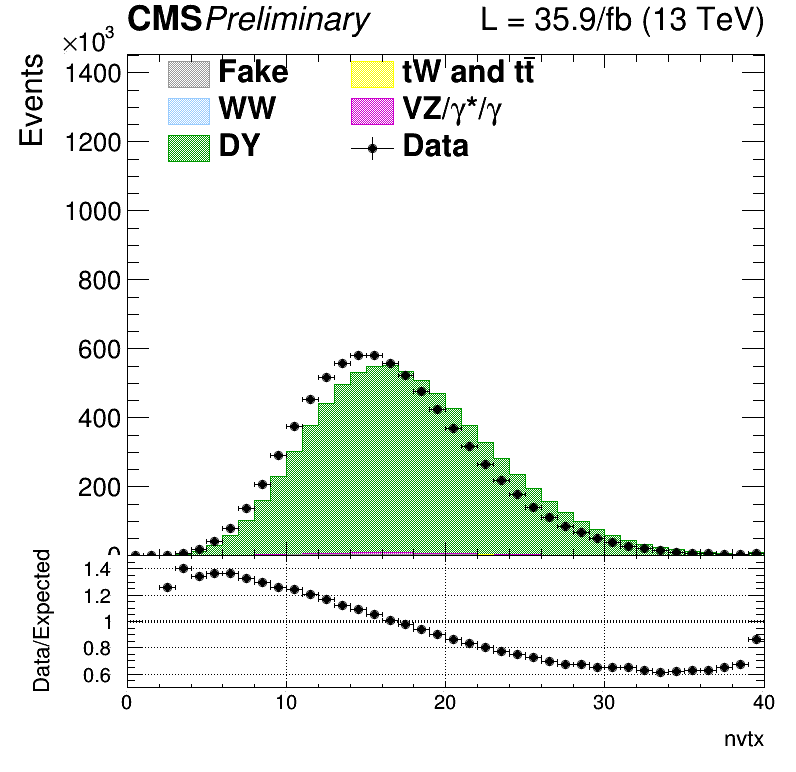
\includegraphics[width=0.6\textwidth]{../AN/Figs/nvertices.png}
\caption{
    Distribution of the number of vertices in a Drell-Yan enriched sample
    (Z$\rightarrow{}ee$) in
    data}
    \label{Fig:pu}
\end{figure*}




\section{Calorimeter clusters}
The purposes of the clustering algorithm in the calorimeters are~\cite{Sirunyan:2017ulk}:
\begin{itemize} 
\item detect and measure the energy and direction of stable neutral particles such as photons and neutral hadrons;
\item separate these neutral particles from charged hadron energy deposits;
\item reconstruct and identify electrons and all accompanying bremsstrahlung photons;
\item help the energy measurement of charged hadrons for which the track parameters were not determined accurately,
which is the case for low-quality and very high $p_T$ tracks.
\end{itemize}
For the PF event reconstruction, a  specific clustering algorithm was developed. 
The clustering is performed separately in each sub-detector: ECAL (barrel and endcaps) and HCAL (barrel and endcaps)
In the algorithm, first, \textit{cluster seeds} are identified   as cells with an energy larger than a given seed threshold, and
larger than the energy of the neighbouring cells. Second, \textit{topological clusters} are grown from the seeds by aggregating cells with at least a corner in common with a cell already in the cluster.
%After an expectation-maximization algorithm based on a Gaussian-mixture mode to
%reconstruct the clusters within a topological cluster is used.
%The Gaussian-mixture model postulates
%that the energy deposits in the M individual cells of the topological cluster arise from N Gaussian energy deposits where N is the number of seeds. 
%The expectation-maximization algorithm is an iterative algorithm with two steps at each iteration.
%During the first step, the parameters of the model are kept constant and the parameters of the model are determined during the second step in an analytical maximum-
%likelihood. 
%The energy and position of the seeds are used as initial values for the parameters of the corresponding 
%Gaussian functions and the expectation maximization cycle is repeated until convergence.

\section{Link algorithm}
A given particle is, in general, expected to give rise to several PF elements in the various CMS
sub-detectors. The reconstruction of a particle therefore proceeds first with a
link algorithm that connects the PF elements from different sub-detectors.
The link between a track in the central tracker and a calorimeter cluster is established as follows:
the track is first extrapolated from its last measured hit in the tracker to
the ECAL at a depth corresponding to the expected maximum of a typical longitudinal electron shower
profile, and to the HCAL at a depth corresponding to one interaction length.  
The track is linked to a cluster if its extrapolated position is within the cluster area, defined by the union of the
areas in the HCAL and the ECAL in $(\phi, \eta)$ plane. 
After, Calorimeter cluster-to-cluster links are sought between HCAL clusters and ECAL clusters.
Charged-particle tracks may also be linked together through a common secondary vertex, for
nuclear-interaction reconstruction.
Finally, a link between a track in the central tracker and information in the muon detector is
established to form global and tracker muons, Sec~\ref{ler}.\\

% In each PF block, the identification and reconstruction sequence proceeds as,
% \begin{itemize} 
% \item first, muon candidates are identified and reconstructed and the
% corresponding PF elements (tracks and clusters) are removed from the PF block.  
% \item The electron identification and reconstruction follows. Energetic and isolated photons, converted or un-
% converted, are identified in the same step.  The corresponding tracks and ECAL or preshower
% clusters are excluded from further consideration
% \item The remaining elements in the block are then subject to a cross-identification of charged hadrons,
% neutral hadrons, and photons, arising from parton fragmentation, hadronization, and decays
% in jets. 
% \end{itemize}


\section{Lepton reconstruction and identification}
\label{ler}
\subsection*{Electron reconstruction and identification}
The combination of tracker and ECAL information is used for electrons reconstruction.
The electrons, emerging from a collision, when interact with the silicon tracker, radiate bremsstrahlung photons that reaches the ECAL with a significant spread in the azimuthal direction $\phi$. These energy deposit measured in ECAL are the starting point of the electrons reconstruction algorithm. They are associated in clusters and in superclusters (clusters of clusters) that take into account the spread in the $\phi$ direction of the bremsstrahlung energy, Fig.~\ref{clustering}.
When   superclusters are identified, the reconstruction algorithm tries to match them to track seeds. The  track seeds are identified as pairs or triplets of hits in the inner tracker layers. The electrons trajectories are reconstructed using a dedicated modeling that take in account  energy
loss in the tracker layers via  bremsstrahlung radiation: non-Gaussian contributions to the event-by-event fluctuations 
of the calorimetry and tracking measurements are introduced due to the bremsstrahlung radiation.   
\begin{figure}
\centering
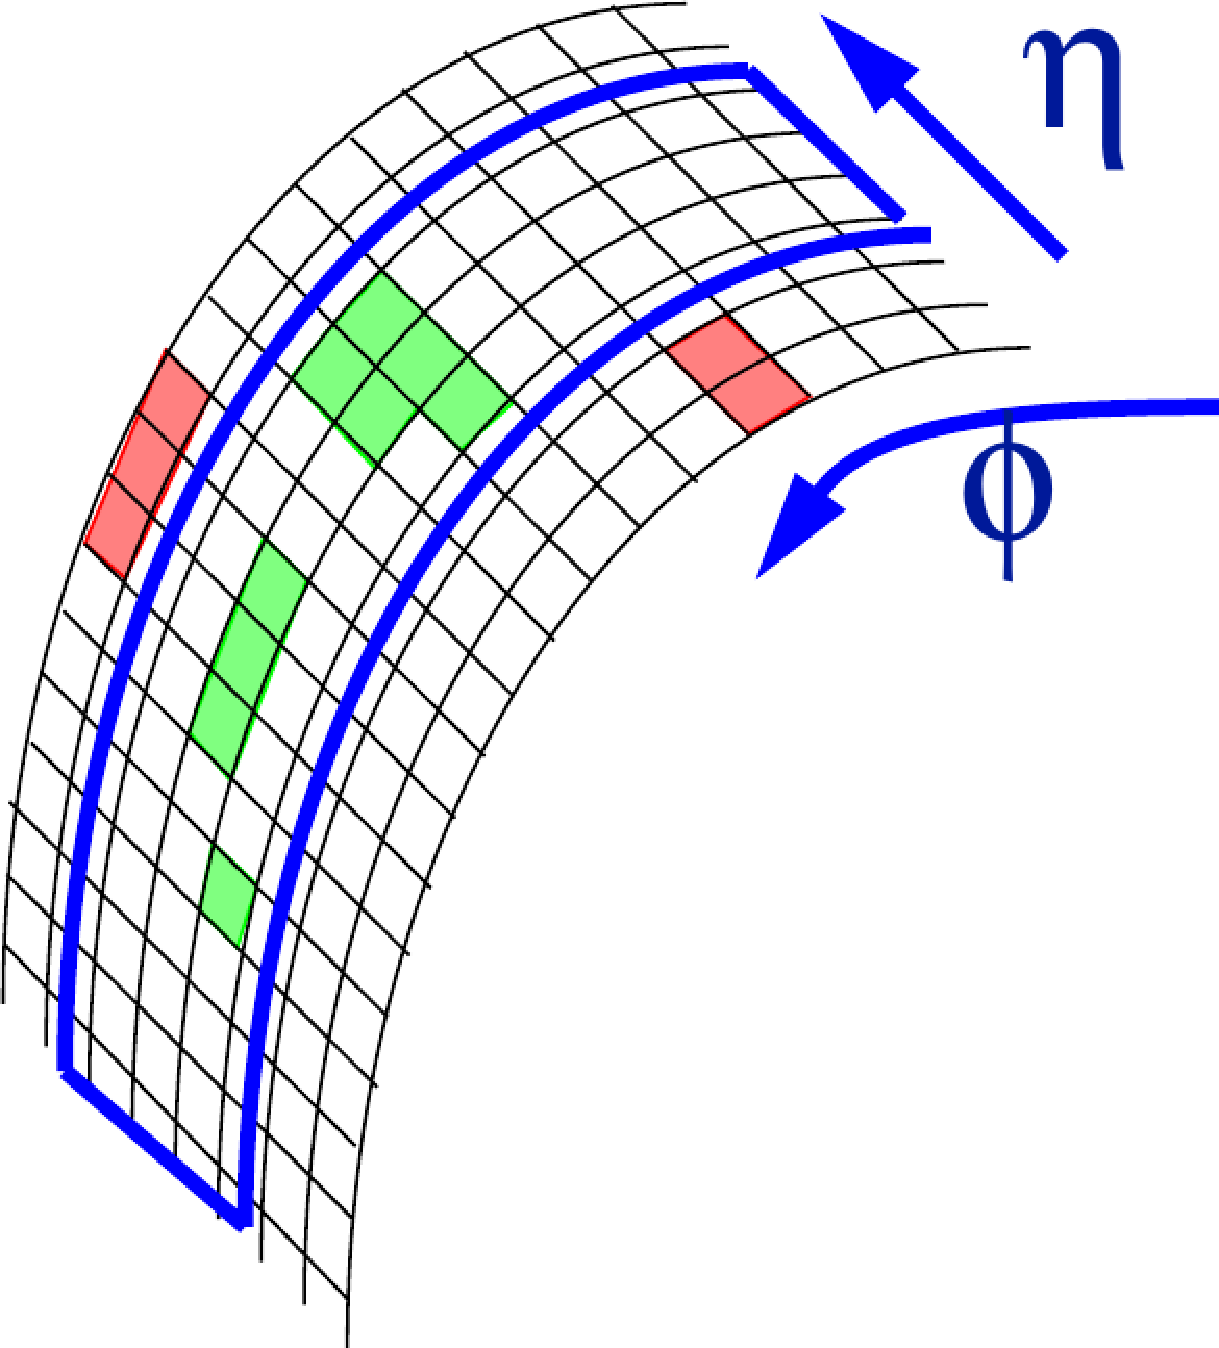
\includegraphics[scale= 0.2]{../Cap4/clustering}
\caption{EM cluster spread in $\eta$ and $\phi$.}
\label{clustering}
\end{figure}
A preselection is applied to solve ambiguous cases where several tracks are reconstructed. It is based on matching
between the GSF track and the supercluster in $\eta$ and $\phi$. To achieve a good resolution the electron supercluster must
be inside the ECAL acceptance volume, meaning that  $|\eta|<$ 2.5, and outside the ECAL barrel-endcap
overlap region, 1.4442 $<|\eta|<$ 1.566.
Several identification variables are used to achieve a good discrimination. These variables are:
\begin{itemize}
\item $\Delta \eta_{trk,SC}$ and $\Delta \phi_{trk,SC}$, that measure the spatial matching between the track
and the supercluster.
\item $\sigma_{in,in}$ that measures the width of the ECAL supercluster in the $\eta$ direction. It is the calorimeter shower shape.
\item H/E: is the ratio among the energy deposit in the HCAL tower and the energy of the seed supercluster.
\item $|$1/E - 1/p$|$ the difference of 1/E measured in ECAL and 1/p measured in the tracker.
\item Number of missing hits
\item $d_{xy}$ and $d_z$, impact parameters with respect to the reconstructed primary vertex (PV).
\item $\gamma \to e^+ e^-$ veto based on missing hits in the inner layers of the tracker.
\end{itemize}
Different selections on the above variables define different working points (WP). The cuts are also different for electrons in
the ECAL barrel or in the endcap. The WPs are:
\begin{itemize}
\item Tight WP: this corresponds to an average 70\% selection efficiency for electrons with
$p_T >$ 20 GeV. This working point is used where backgrounds are very large. The
$X \to WW$ high mass analysis has large backgrounds like W+jets, where the second lepton is a ``fake'', i.e. a jet identified as an isolated lepton. 
So, in this analysis we use Tight WP for electrons. %On the top of that, we apply more cuts to make the electron id selection Trigger safe.
\item Medium WP: the average efficiency is about 80\% for electrons with $p_T>$ 20
GeV. This is also a good starting point for measurements of W and Z cross-sections.
\item Loose WP: this working point is used only for very clean final states. The average efficiency is about 90\%.
\item Veto WP: generally, this is not used for signal selection. However, it is found to
be useful for extra lepton veto counting of electrons. The average efficiency is about 95\%.
\end{itemize}
Selected electrons are also required to pass the isolation criteria that include a pile-up mitigation correction based on the electron effective 
catchment area. The isolation variable is computed for each electron as,
\begin{equation}
ISO^{Rel}_{EA\; corrected}=[\sum_{ChH}(p_T) + max(0, \sum_{Ph}(p_T)) +\sum_{NH}(p_T)  -\rho EA ]/p_T^{electron} \, ,
\end{equation}
where $ChH$ is an index which runs on the charged hadrons, $Ph$ on the photons, $NH$ on the neutral hadrons, $\rho$ is the pile up energy
density and $A$ is an effective area. The sum is done in a isolated cone of $\Delta R<$ 0.4 around the electron direction.
The identification and isolation criteria used for the $X \to WW$ analysis are summarised in Tab.~\ref{IDe}.
\begin{table}
\centering
\begin{tabular}{|lll|}
\hline
Observable & Barrel (EB) cut &Endcap (EE) cut\\
\hline
$|\Delta \eta_{trk,SC}|$  &0.00308  & 0.00605 \\
$|\Delta \phi_{trk,SC}|$ & 0.0816   &0.0394\\
$\sigma_{in,in}$ &0.011& 0.031\\
H/E & 0.060& 0.065\\
$|$1/E - 1/p$|$ & 0.013 &0.013\\
Number of missing &1&1\\
$|d_{xy}|$ &0.05&1\\
$|d_z|$ &1&1\\
conversion veto& true&true\\ 
\hline
$ISO^{Rel}_{EA\; corrected}$&0.0588 & 0.0571\\
\hline
\end{tabular}
\caption{Electron identification criteria for the Tight working point and isolation requirements.}
\label{IDe}
\end{table}

\subsection*{Muon reconstruction and identification}
Muons produced in the interaction point can pass through all the detector, with a negligible energy loss, and give a signal in the muon chambers.
%Their loss of energy is very negligible. 
They are thus seen both in the silicon tracker and in the external muon chambers. 
The reconstruction starts from the measurements of DT, CSC and RPC sub-detectors. This reconstructed track in the muon spectrometer is called
Stand-alone Muon.
In parallel, muon tracks are also reconstructed in the inner silicon tracker, as described before for generic charged particles.
%Seeds are
%built using two or three consecutive hits in the pixel and or in the strip detector. 
%The pattern recognition is performed starting from these seeds and proceeding layer by layer,
%with an iterative technique based on the Kalman Filter.
%At the end of this algorithm, a track fit is performed and the track parameters are updated. 
The tracker track is then combined with the Stand-alone Muon track in order to construct
a global track, which defines a Global Muon. A global fit is performed for each pair of
tracks reconstructed in the inner tracker and in the muon system. If more than one track
matching the stand-alone track is found, then the one giving the best $\chi^2$ in the global fit
is chosen. A complementary approach consists in considering all tracker tracks with $p_T>$ 0.5 GeV as
potential muon candidates. These tracks are extrapolated to the muon system taking
into account the magnetic field. If at least one muon segment (a short track stub made of
DT or CSC hits) matches the extrapolated tracks, the corresponding tracker track is
identified as a Tracker Muon.
Quality requirements are applied to ensure a good quality of the reconstruction:
\begin{itemize}
 \item the tracker track has to be reconstructed from at least 5 tracker layers with hits; 
 \item at least one hit must be present in the pixel detector;
 \item at least one hit must be present in the muon detector;
 \item at least one muon chamber hit should be included in the Global Muon track fit;
 \item the normalized $\chi^2$ of the Global Muon track fit should be less than 10;
 \item the muon track reconstructed in the tracker must have a distance to the primary
vertex smaller than 2 mm in the transverse plane and smaller than 5 mm in
the longitudinal direction.
\end{itemize}
The requirements are summarized in Tab.\ref{IDm}.
\begin{table}
\centering
\begin{tabular}{|ll|}
\hline
Observable& Value Cut\\
\hline
Is global muon                        & true              \\ 
Is PF muon                            & true              \\ 
Tracker layers with measurements      & $>5$              \\ 
Number of valid pixel hits            & $>0$              \\ 
Number of valid muon hits             & $>0$              \\ 
Number of matched muon stations       & $>1$              \\ 
$\chi^2$ /ndof                        & $<10$             \\ 
$d_{xy}$ (PV)                         & < 0.2 cm          \\ 
$d_z$ (PV)                            & < 0.5 cm          \\ 
\hline
$ISO^{Rel}_{\Delta \beta}$              & $<$0.15\\
\hline
\end{tabular}
\caption{Muon identification and isolation requirements.}
\label{IDm}
\end{table}
For the analysis goals, the muons are expected to be isolated, as the they are generated by W boson decay. 
Indeed, muons produced by W or Z boson decay, or prompt muons, are expected to be isolated in the event, contrary to non-prompt muons, muons from in flight decays, that are generally produced within jets and characterized by many
nearby particles. Muons coming from $W$s are therefore requested to pass an isolation
criterion, which includes a PU mitigation, called ``$\Delta \beta$ correction'',
%Indeed the isolation variable is sensitive to the
%pileup and a correction is applied 
in order to ensure its independence and robustness on
the number of simultaneous interactions. The isolation variable used is,
\begin{equation} 
ISO^{Rel}_{\Delta \beta}=[\sum_{ChH}(p_T) + max(0, \sum_{Ph}(p_T) -0.5 \times \sum_{ChHUP}(p_T)) ]/p_T^{electron} \, ,
\end{equation}
where $ChH$ is the charged hadrons, $Ph$ is photons and $ChHPU$ is charged
hadrons not coming from the primary vertex.  The sum is performed in a cone of 0.4 units in $\Delta R$ around the muon
and the $ISO^{Rel}_{\Delta \beta}$ cut is 0.15
A bias in the muon $p_T$ is introduced by the imperfect knowledge
of the magnetic field and the effect of the material distribution. In addition the $p_T$ measurement is sensitive to the alignment of the tracker and
muon chambers. To estimate the muon $p_T$ scale and resolution 
%different methods have been developed. For $p_T<100$ GeV,  
events with two muons from a $J/\Psi$ or a Z
resonance decay are used. 
%Above, so in the high $p_T$ regime, cosmic ray muons are  to correct the $p_T$ scale.

\section{Jet reconstruction and identification}
\label{jetr}
Jets are the experimental signature of quarks and gluons produced in the hadron collision. They result from the parton  hadronization and they play a major role in a hadronic collider where processes with jets in the final state have very large cross-section. %The technique used for jet reconstruction is the Particle Flow.
Using the particle-flow algorithm described in Sec.~\ref{PFt}, the  jets are reconstructed by clustering of the  four-momentum vectors of PF candidates.%: the information from relevant CMS sub-detectors are used to identify and to reconstruct all visible particles in the event, as
% muons, electrons, photons, charged hadrons, and neutral hadrons. 
The momentum and spatial resolutions of these jets reconstructed with the PF technique are greatly improved with respect to jets obtained using the calorimeters information only, because the tracking detector allows a better resolution of $p_T$ for the charged particles.
The four-vectors of input particles are combined with a sequential and iterative jet clustering algorithm, that should have ideally the following features:
\begin{itemize}
\item infrared safety: no infrared singularity appears in perturbative calculations for the results of this algorithm;
\item collinear safety: same as before for collinear singularities;
\item invariance under boosts: the algorithm should find the same solutions independently
by boosts in the longitudinal direction.
\item order independence: the algorithm should find the same jets at parton, particle, and detector level;
\item straightforward implementation: the algorithm should be straightforward to implement in perturbative calculations.
\end{itemize}
The jet algorithm should also follow these  experimental criteria:
\begin{itemize}
\item detector independence: the performance of the algorithm should be independent from the detector;
\item minimization of resolution smearing and angle biases: the algorithm should not
amplify the inevitable effects of resolution smearing and angle biases;
\item stability with luminosity: jet finding should not be strongly affected by pileup;
\item efficient use of computing resources: minimum  computer time consumption;
\item maximal reconstruction efficiency: the algorithm should efficiently identify all jets;
\item ease of calibration and use: algorithm should not obstruct a reliable calibration and be straightforward to implement.
\end{itemize}
Jet definition is not unique, being the parton not a well-defined objects, from the experimental point of view, so several
approaches for jet clustering are available. Two main algorithms have been developed: the ``conical recombination'' algorithm
that puts together particles within specific conical angular regions, notably such that
the momentum sum of the particles contained in a given cone coincides
with the cone axis (a ``stable cone'') and
the ``sequential recombination'' algorithm   that works by defining a distance
between pairs of particles, then performing subsequent recombinations of pairs of closest
particles, and stopping when all resulting objects are too far apart. The standard algorithms adopted by
CMS are the SISCone in the conical recombination class, and the $k_t$, Cambridge-Aachen (CA) and anti-$k_T$ algorithms for the sequential, Sec~\ref{rico_jet}.\\
\newline
\subsection*{Jet Energy Calibration}
The purpose of the jet energy calibration is to relate, on average, the energy measured for the
detector jet to the energy of the corresponding true particle jet.  A true particle jet results from
the clustering (with the same clustering algorithm applied to detector jets, Sec.~\ref{jetr}) of all stable particles
originating from the fragmenting parton, as well as of the particles from the underlying event
(UE) activity. \\
The jet energy calibration is related,  on average, on the energy measured in
the detector to the true energy of the corresponding final state particle jet or parton jet.
From the clustering  of all stable particles, a true particle jet results. The correction is applied as
a multiplicative factor C to each component of the raw jet four-momentum vector, $p_{\mu}^{raw}$, as:
\newline
\begin{equation}
p_{\mu}^{corr}=C \cdot p_{\mu}^{raw} \; ,
\end{equation}
where correction factor $C$ is composed of the offset correction $C_{offset}$ , the MC calibration
factor $C_{MC}$, and the residual calibrations $C_{rel}$ and $C_{abs}$ for the relative and absolute
energy scales, respectively. The various components are applied in sequence:
\newline
\begin{equation}
C=   C_{offset} ( p_{\mu}^{raw}) \cdot  C_{MC} (p_T',\eta) \cdot C_{rel}(\eta) \cdot  C_{abs} (p_T'') \; ,
\end{equation}
\newline
where $p_T'$ is the transverse momentum of the jet after applying the offset correction and $p_T''$ is the transverse momentum 
of the jet after all previous corrections. The details of each component are:
\begin{itemize}
\item $C_{offset}$: a energy offset is produced by the pileup of multiple proton-proton collisions and by electronic noise.
The goal of the offset correction is to subtract, on average, the unwanted
energy from the jet. For the offset correction estimation, the Jet Area Method has been used~\cite{Cacciari:2007fd}. 
% An average $p_T$-density $\rho$ per unit area is estimated, for each event. 
% The key element for this approach is the jet area $A_j$.
% A very large number of infinitely soft four-momentum vectors are artificially added in the event and clustered
% by the jet algorithm together with the true jet components. The other important quantity for the pileup subtraction is the $p_T$ density $\rho$, which
% is calculated with the $k_T$ jet clustering algorithm with a distance parameter R$=$0.6.
% The quantity $\rho$ is defined on an event-by-event basis as the median of the distribution of
% the variable $p_{Tj}  /A_j$ , where j runs over all jets in the event, and is not sensitive to the
% presence of hard jets. Therefore, the event-by-event and jet-by-jet offset correction can be defined as,
% \begin{equation}
%   C_{offset}= (p_T^{raw}, A_j ,\rho )=1- \frac{(\rho -\langle \rho_{UE}  \rangle )\cdot A_j }{p_T^{raw}} \; ,
% \end{equation}
% where $\langle \rho_{UE}  \rangle$ is the $p_T$-density component due to the UE and electronics
% noise, and is measured in events with exactly one reconstructed primary vertex (no pileup).
\item $C_{MC}$: is based on the simulation and corrects the energy of the reconstructed
jets such that it is equal on average to the energy of the generated jets (GenJets). The
GenJets reconstruction algorithm is identical to the one applied to the data.
The response variable, $R=p_T^{reco}/p_T^{gen}$, in each bin of the GenJet transverse momentum $p_T^{gen}$, is recorded as jet $p_T^{reco}$.
The average correction in each bin is defined as,
\begin{equation}
  C_{MC}(p_T^{reco})= \frac{1}{\langle R \rangle } \; ,
\end{equation}
\item $C_{rel}$: the goal of the relative jet energy scale correction is to make the jet response flat versus $\eta$. 
%This is achieved by employing a Tag and Probe technique, selecting dijet
%events in data.
The size of this residual correction is of the order of 2-3\% in the
central $\eta$ region, while it goes up to about 10\% in the forward region.
\item $C_{abs}$: the goal of the absolute jet energy scale correction is to make the jet response flat versus $p_T$.
Once a jet has been corrected for $\eta$ dependence, it is corrected back to particle
level.
\end{itemize}
Each type of correction has uncertainties arising from many different sources.
These sources are categorized as: physics modeling in MC, MC modeling of true detector response and potential biases in the methodologies used to estimate the corrections. In CMS more than 16 such sources of uncertainties have been identified. Several are
related and can be combined into groups that are relative to the absolute scale, relative
scale, extrapolation in $p_T$, pileup, jet flavor and time stability.
% \section{Pileup subtraction}
% % in fact for the  neutral particles it is not possible to distinct primary vertex that corresponds to a single
% %roton-proton interaction,  and most jet measurements are carried out with calorimeters, which do not have the angular
% %resolution needed to reconstruct the original primary vertex.\\
% An event-by-event, and jet-by-jet, pileup subtraction approach, which performs the corrections after the jet finding,  is carried out~\cite{Cacciari:2007fd}.  It is based on:
% \begin{itemize}
% \item the jet’s susceptibility to contamination: it is embodied in the jet area A measured on $\eta$ and $\phi$. The jet area is different for each jet and depends on the details of its substructure, and practical measurement of the jet areas is carried out using the FastJet package. 
% Given a suitable definition of jet area, the modification of a jet’s $p_T$ by diffuse noise can be shown to be,
% \begin{equation} 
% \Delta p_T=A\rho \pm \sigma \sqrt{A} -L \:, \qquad \langle L \rangle=\mathcal{O}(\alpha_S \times A \rho \ln \frac{p_T}{ A \rho}) \:,  
% \end{equation} 
% where $\rho$ is the level of diffuse noise that  corresponds to the amount of transverse momentum added to the event per unit area (at LHC is around 
% 10-20 GeV~\cite{Sjostrand:2003wg}): the first term is therefore the geometrical contamination of the je
% t and is associated with an uncertainty (second term) because of fluctuations in the noise from point to point in the event.
% $L$  accounts for the occasional loss (or the even more occasional gain) of part of the jet’s contents,
% due to the fact that jets can be modified when clustered in the presence of diffuse noise, as some
% of the particles originally clustered into one jet can instead end up in a different one. \\
% If the fluctuations are small, $\sigma << \sqrt{A} \, \rho$, the measured $p_T$ for each jet $j$ using the subtraction is given by,
% \begin{equation} 
% p_{T,j}^{sub}=p_{T,j} -A_J \rho \: ,
% \end{equation} 
% where $A_j $ is the jet area. This equation provides a correction to the jet’s scalar transverse
% momentum.
% \item The second ingredient in carrying out the subtraction is the estimate of $\rho$ for each event.
% The principal difficulty in estimating the amount of noise is that of distinguishing the noise component from the large amounts of $p_T$ deposited by the hard event.
% The $\rho$ value  for each even can be estimated~\cite{Cacciari:2007fd}  taking the median value of this distribution in the event: 
% \begin{equation} 
% \rho= median \; [\{\frac{p_{T,j}}{A_j}\}]  \: ,
% \end{equation} 
% \end{itemize}
% The above pileup subtraction procedure is valid if: 
% \begin{itemize}
% \item The pileup noise should be independent of $\eta$ and $\phi$.
% \item The radius $R$ of the jet algorithm should be no smaller than the typical distance between minimum bias particles, otherwise the extraction of
%  $\rho$ from the median will be biased by the large amount of empty area not associated with jets
% \item The number of pileup jets should be much larger than the number of jets from the hard interaction. 
% \end{itemize}

\subsection*{Jets in $X \to WW$ analysis}
%The jets collection is made by clustering the reconstructed particles known as the Particle Flow
%candidates. 
The clustering algorithm used for jet reconstruction in the $X \to WW$ analysis is the anti-kt algorithm with
a distance parameter equal to 0.4. Pileup mitigation is done with the Charge Hadron Subtraction  algorithm~\cite{CMS-PAS-JME-14-001} 
which removes charged particles coming from pileup vertices before
clustering.
%The Jet Energy Corrections  that are applied to correct the reconstructed jet energy back
%to the true energy of the final state particles. 
To reject jets originating
from calorimeter or readout electronics noise the loose working point of the PF Jet Identification is applied. 
This analysis selects jets with
\begin{equation}
 p_T^{Jet} > 30 \, \mathrm{GeV} \: , |\eta| < 5.0 \: .
\end{equation}
Kinematic distributions of the jets after applying corrections are shown in Fig.~\ref{jetFig} for a Drell-Yan enriched sample.  As can be seen from the plot there is a reasonable agreement between simulation and data. The residual discrepancies are covered by the uncertainties of the jet energy corrections (Sec.~\ref{jetr}) which are not shown in the plots.
%\begin{figure}
%\centering
%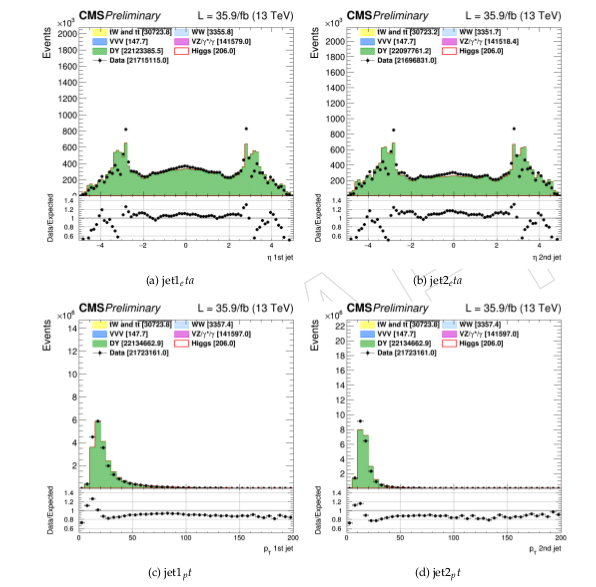
\includegraphics[scale= 0.5]{../Cap4/jetFig}
%\caption{The jet kinematic distributions}
%\label{jetFig}
%\end{figure}

\begin{figure}[htbp]
 \captionsetup[subfigure]{margin=1pt}
 \centering
    \subfigure[$\eta$ jet1 ]{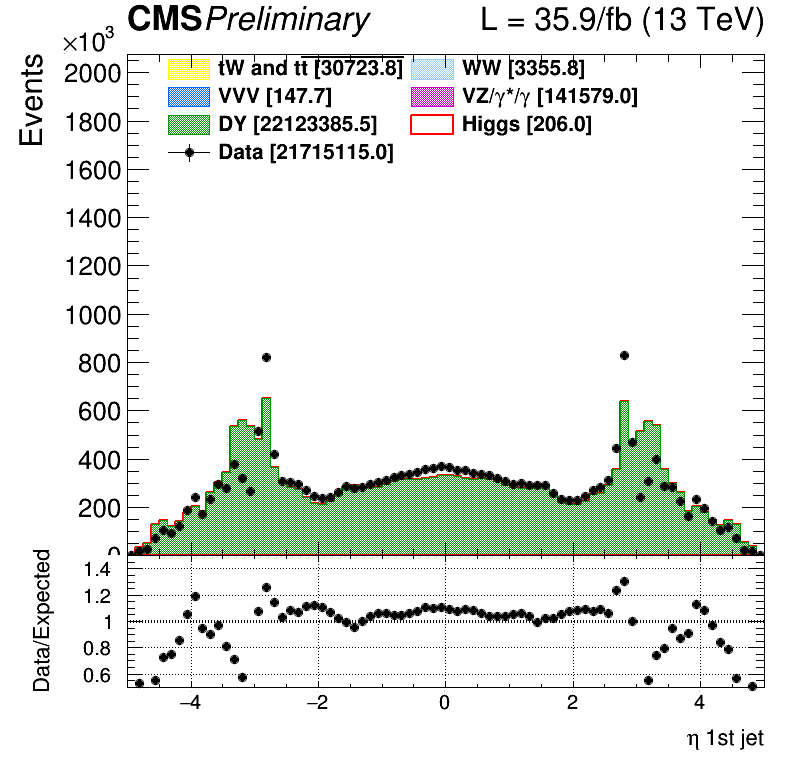
\includegraphics[width=0.45\textwidth]{../Cap4/Figs/Jet/cratio_Zmm_jeteta1.png}}
    \subfigure[$\eta$ jet2]{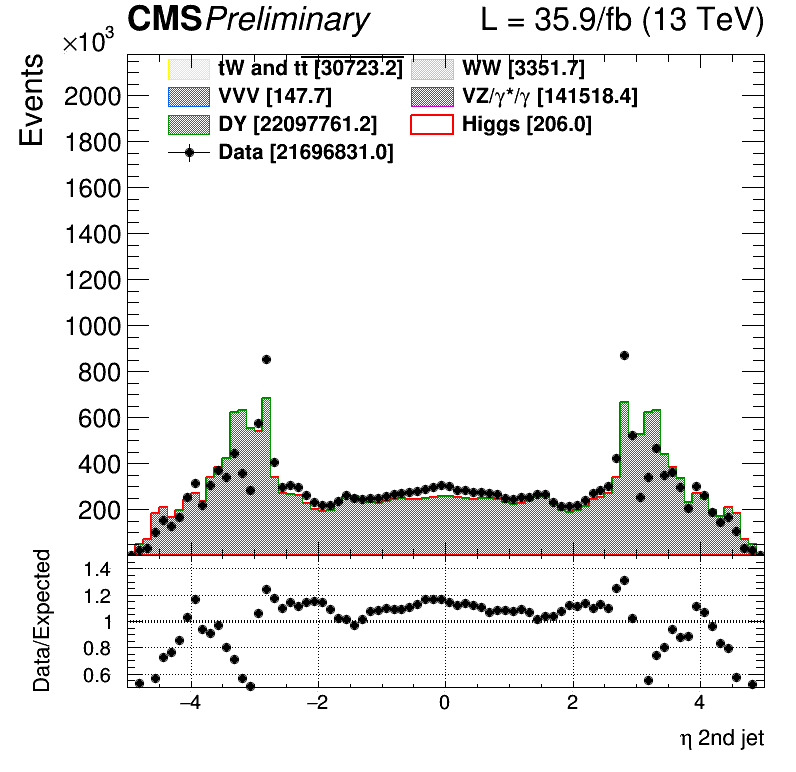
\includegraphics[width=0.45\textwidth]{../Cap4/Figs/Jet/cratio_Zmm_jeteta2.png}}
    \\
    \subfigure[$p_T$ jet1]{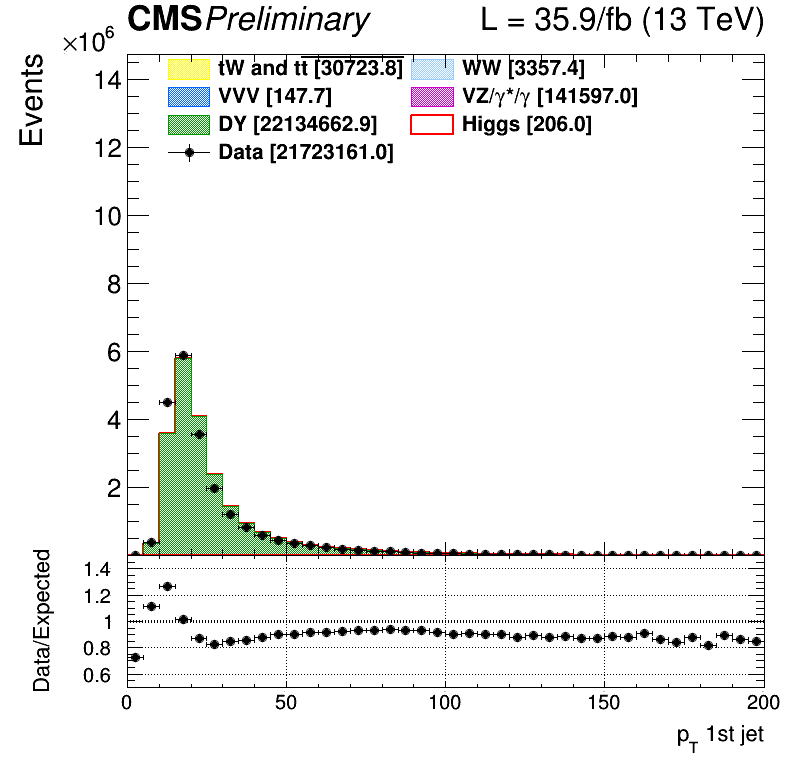
\includegraphics[width=0.45\textwidth]{../Cap4/Figs/Jet/cratio_Jet_13TeV_of_jet1_pt.png}}
    \subfigure[$p_T$ jet2]{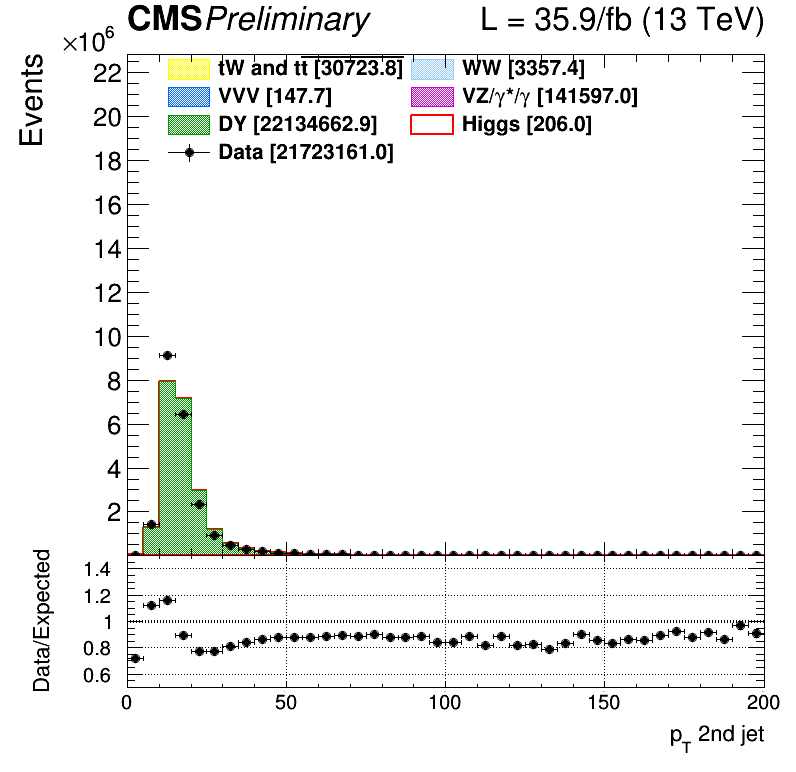
\includegraphics[width=0.45\textwidth]{../Cap4/Figs/Jet/cratio_Jet_13TeV_of_jet2_pt.png}}
    %\subfigure[jet3_pt]{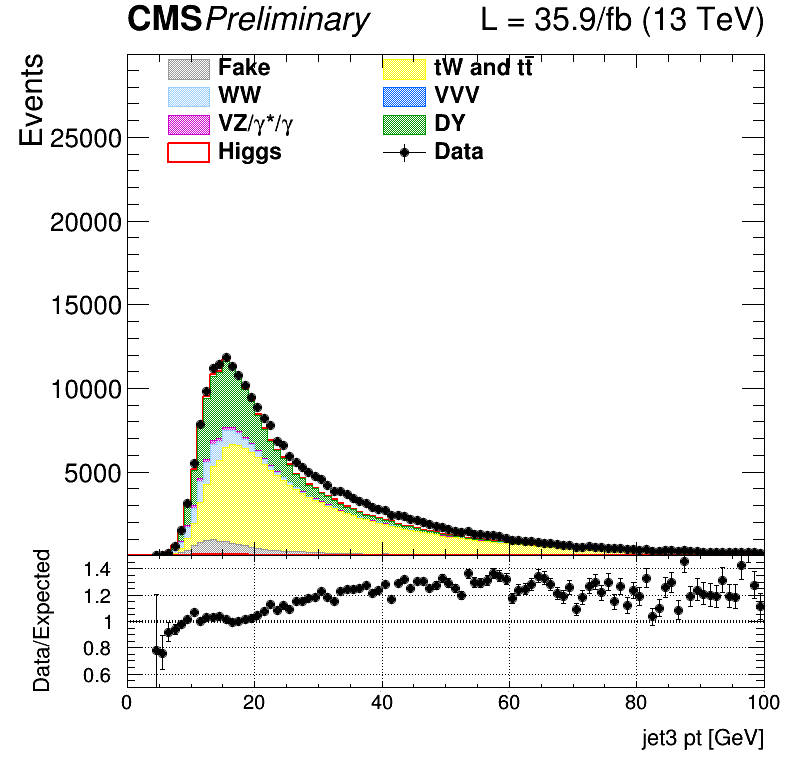
\includegraphics[width=0.45\textwidth]{Figs/Jet/cratio_Jet_13TeV_of_jet3_pt.png}\label{fig:jet3_pt}}
    \caption{
      The jet kinematic distributions ($\eta$ and $p_T$) for the first and for the second jet. }
%\label{jetFig}
\end{figure}


\section{b-jet identification}
To identify the b jets, the peculiarities that characterize hadrons
containing the quark b are used.
These hadrons have a relatively large mass, around 5 GeV, and a long lifetime, of about 1.5 ps. Given that they can
have an impulse of several tens of GeV, the distance that they travel in the detector
it is of the order of:
\begin{eqnarray}
  \delta &\approx& \langle t \rangle \: v \approx \gamma \: \tau \: \beta  \: c  \nonumber \\
 &\approx& 10 \cdot 1.5 \cdot 10^{-12} \mbox{s} \cdot 1 \cdot 3 \cdot 10^8 \: \mbox{m/s}   \nonumber \\
 &\approx& 5  \mbox{mm,} \end{eqnarray}
a distance that can be measured since the accuracy of the position of the
secondary vertices is $\sim$100 $\mu$m.
The CMS collaboration has developed different algorithms to identify the jets coming from
  quarks b (b-tag algorithms)~\cite{Chatrchyan:2012jua}. Each of these algorithms is characterized
by the efficiency of signal identification (i.e. to select jets from b quark) versus the probability of
rejecting the background (jets that are not from b quark), which in general depend on the transverse impulse,
$p_T$, and on the pseudorapidity of the jet. To build an observable (or discriminator) which can separate 
jets originated by b from those originating from light quark 
reconstructed objects such as tracks, vertices and leptons are used.
Some simple algorithms use a single observable in input, while others,
more complexes, combine several variables. Each algorithm
produces, in output, a value of the discriminator for each jet of the event.
The first step in identifying of b-jets is the reconstruction of all the jets in the
the event, using, as mentioned, the anti-$k_T$ algorithm. However b-jet
identification algorithms require a sample with well reconstructed and high purity tracks.
Therefore further cuts to the tracks in the jet are applied. First of all, to reduce
the number of tracks reconstructed incorrectly, transverse momentum must be 
greater than 1 GeV and at least two hits must be present in the silicon pixel detector. Then, at 
least eight hits per each track must be present and the fit must have 
 $\chi^2$/d.o.f. $<$5, where d.o.f. it is the number of degrees of freedom.
A selection is also applied on the impact parameter (see below): this is used to increase
the fraction of well reconstructed tracks and to reduce the contamination due to long life particles like neutral kaons.
The transverse distance $d_{xy}$ and longitudinal $d_z$ between the track and the primary vertex
are required to be smaller than 0.2 cm and 17 cm respectively.
In Fig.~\ref{bj},  
a schematic representation of the parameters used in the identification 
of the b jets is given.
\begin{figure}
\centering
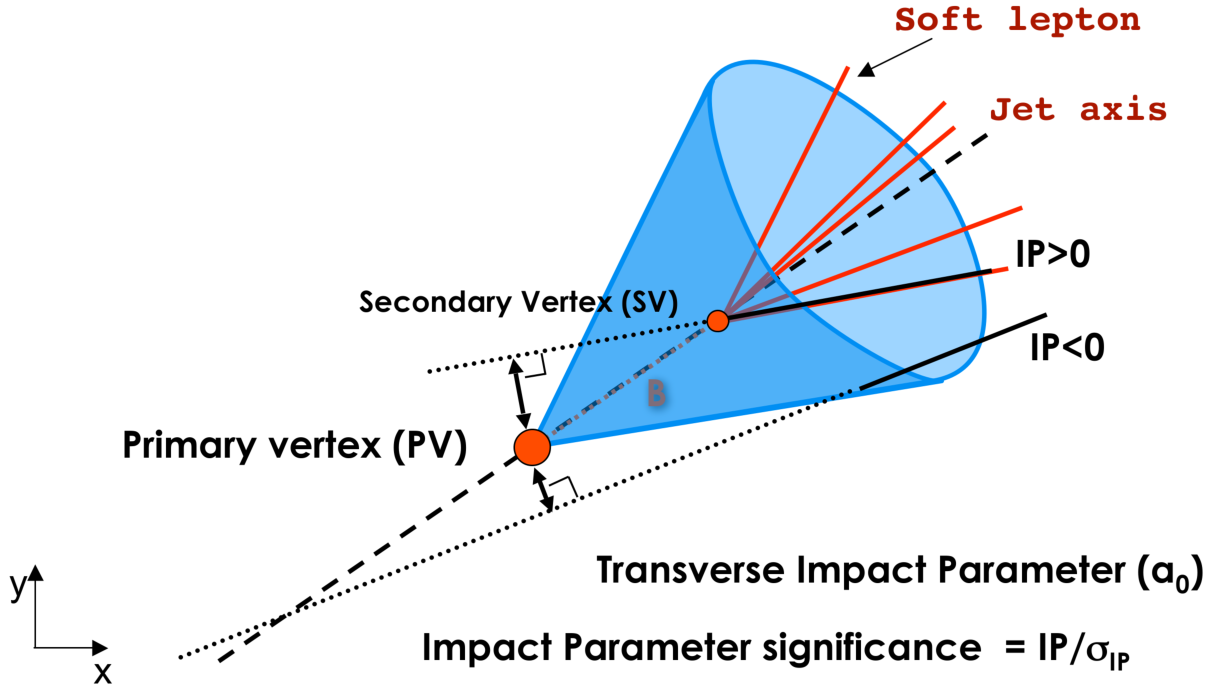
\includegraphics[scale= 0.5]{../Cap4/btag}
\caption{Cluster spread in $\eta$ and $\phi$.}
\label{bj}
\end{figure}
\subsection*{Impact Parameter algorithm}
The impact parameter (IP) of a track respect to the primary vertex, can be used to distinguish 
the hadrons b decay  respect to background tracks (prompt). The IP is calculated in three dimensions 
thanks to the excellent resolution of the pixel detector.
The impact parameter has the same sign of the scalar product between the direction of the
jet and the vector between the primary vertex and the nearest point of the track. The tracks
due to the decay of a hadron with a long lifetime
have a positive IP, while for tracks originated from the primary vertex
the IP is equally negative or positive.
The variable used as observable is the significance of the impact parameter, 
S$_{IP}$, defined as the ratio between IP and its estimated uncertainty.
% There
%significance of the impact parameter can therefore be used as a discriminant  between b and non-b jets.
The Track Counting (TC) algorithm orders according to their IP significance
the tracks of the jet, from the highest to lowest. There are two versions of this algorithm that
differ for which value of the IP significance is used as the discriminator:
Track Counting High Efficiency (TCHE) uses the S$_{IP}$ of the second track, while the Track Counting High Purity (TCHP) uses the third.
A natural extension of the TC algorithms is the combination of the several tracks impact points. 
This is implemented in the Jet Probability (JP) and Jet
B Probability (JBP) algorithms. The former uses an estimator for the likelihood that 
all the tracks in the jet come
from the primary vertex of the interaction. This estimator, P$_{jet}$, is defined as,
\begin{equation}
P_{jet}=\Pi \cdot \sum_{i=0} ^{N-1} \frac{(-\ln \Pi)^i}{i!} \qquad \mbox{con} \qquad \Pi= \prod_{i=0} ^{N}\mbox{max}(P_i, 0.005)  \mbox{,}\end{equation} 
where N is the number of tracks considered and P  the probability that the track is
originated in the primary vertex.
Instead the JBP algorithm gives more weight to the tracks (up to a maximum of four) that have a high 
value of the IP significance. 

\subsection*{Secondary Vertex identification}
The presence of a
secondary vertex in the event and related variables  can be used
to discriminate jets coming from a quark b respect to the others. The main variables associated with the secondary vertex are the distance, the flight direction
with respect to the primary vertex, the invariant mass and the energy of the tracks associated to 
secondary vertex. To identify a secondary vertex it is required that:
\begin{itemize}
\item less than 65\% of its tracks are associated with the primary vertex and
the significance of the radial distance between the two vertices is beyond 3$\sigma$;
\item the flight distance of each candidate is in a cone of $\Delta R <$0.5 around
the jet direction;
\item it has not a radial distance of more than 2.5 cm from the primary vertex and a mass compatible with
that of K$_0$ or exceeding 6.5 GeV (this is needed to reduce contamination from long-lived mesons and interactions with the detector material).
\end{itemize}
The Simple Secondary Vertex (SSV) algorithm uses as a discriminating variable 
the significance of the flight distance, given by the ratio of the flight distance to its uncertainty. 
Similar to the TC algorithm, there are two versions
of SSV: High Efficiency (SSVHE) which uses vertices to which there are at least
two associated tracks, and High Purity (SSVHP) that requires at least three associated tracks.
%There are more complicated algorithms that consider the secondary vertices together with the
%information on the lifetime. This makes possible to construct a discriminant
%even when there is no secondary vertex, increasing efficiency with respect to 
%SSV; two of these algorithms are the Combined Secondary Vertex (CSV) and the
%Combined Secondary Vertex Version 2 + Inclusive Vertex Finder (CSVV2IVF).
%The difference between the two is that the CSV algorithm uses information from the jets only to reconstruct the vertices while the CSVV2IVF algorithm uses
%all the tracks present in the event.
%In addition there are some other variables that
%can be used to increase the discrimination power
%\begin{itemize}
%\item the category of vertices;
%\item the significance of the flight distance in the transverse plane;
%\item the mass of the vertex;
%\item the number of vertex tracks;
%\item the ratio between the energy carried by a track and the other jet tracks;
%\item the pseudorapidity of the track;
%\item the number of tracks in the jet.
%\end{itemize}

\subsection*{Combined MVA algorithm}
Another class of   b-jet  algorithms is obtained combining several discriminating variables using multivariate algorithms.
One of these  identification algorithms, the  Combined MVA v2 (CMVA), uses the discriminators described previously (JP and SSV) together with 
 Soft Electron (SET) and Soft Muon (SMT) taggers:
the SET algorithm looks for a reconstructed electron inside the jet cone $\Delta R<0.4$;
the SMT algorithm searches for a muon with a transverse momentum of at least 2 GeV among the jet constituents. 
All these inputs are combined used a Boost Decision Tree (BDT) providing a better discrimination with respect to each variable alone.


\subsection*{b-tag performance in $X \to WW$ analysis}
In order to assess which tagger and working point are performing better, we have calculated
the signal significance for different taggers and working points in events with 0 or 1 jet with $p_T>$30  GeV, 
which are the most sensitive to the dominant gluon fusion production mode. In events with 0 jets with $p_T>$30  GeV, the b-tag algorithm is applied to jets with 20$< p_T <$30 GeV, if any. The significance
has been computed running the full analysis for the Standard Model Higgs at 125 GeV~\cite{CMS-PAS-HIG-16-042},  but including only the systematic uncertainties
associated to the b-tagging~\cite{Chatrchyan:2012jua}. The results are shown in Tab.~\ref{btt}.
The results show that the usage of CMVA (loose WP) or  CSV (medium WP) leads to a
comparable signal significance in the combined 0+1 jet category. The CMVA tagger with loose
WP has been found to be the best option for the analysis, given the good performance and the
nice agreement that has been observed between data and MC, Fig.~\ref{cmvaT} and  Fig.~\ref{cmvaD}.

\begin{table}[htb]
\caption{Signal significance for different taggers and working points in the 0 and 1 jet categories. The significance for the combination of the 0 and 1 jet categories is shown as well. Only the systematic uncertainties associated to the b tagging scale factors are taken into account for the significance evaluation.}
\centering
\begin{tabular}{|c|c|c|c|}
\hline
\multirow{2}{*}{Tagger (WP)} & \multicolumn{3}{c|}{Significance} \\
                        & 0 jet & 1 jet & 0+1 jet \\
\hline
CMVA (loose)     & 7.31 & 4.86 & 8.76 \\
CMVA (medium)    & 7.39 & 4.52 & 8.66 \\
CMVA (tight)     & 7.35 & 4.16 & 8.44 \\
\hline
CSV (loose)      & 7.12 & 4.64 & 8.47 \\
CSV (medium)     & 7.37 & 4.47 & 8.62 \\
CSV (tight)      & 7.36 & 4.15 & 8.45 \\
\hline
\end{tabular}
\label{btt}
\end{table}






\begin{figure}
\centering
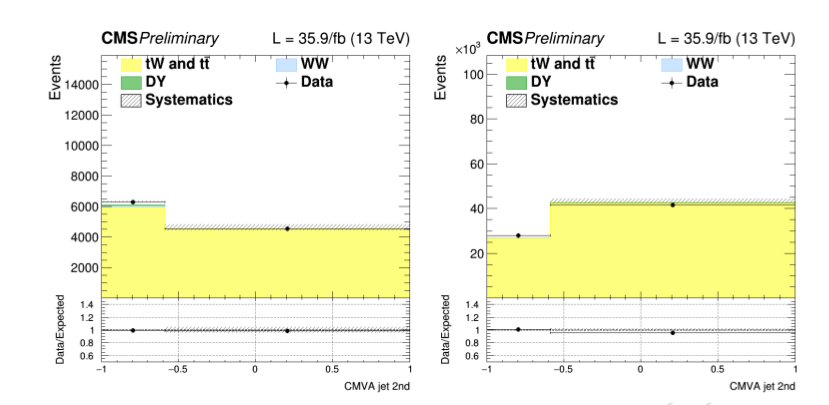
\includegraphics[scale= 0.4]{../Cap4/cmvaT}
\caption{CMVA discriminator for jets above 30 GeV (a) and between 20 and 30 GeV (b) in a
top enriched control region, after applying the scale factors. The top background normalization
is scaled to match data. The systematics band comprises only the uncertainties related to the b-tagging.}
\label{cmvaT}
\end{figure}

\begin{figure}
\centering
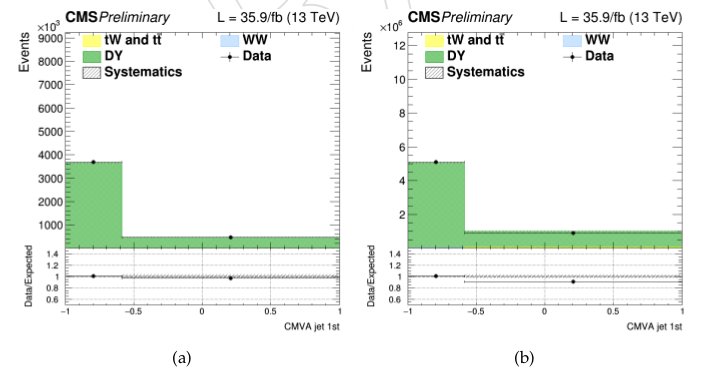
\includegraphics[scale= 0.4]{../Cap4/cmvaD}
\caption{CMVA discriminator for jets between 20 and 30 GeV (a) and above 30 GeV (b) in the
Z enriched control region. The normalization of the DY background is scaled to match data.
The systematics band comprises only the uncertainties related to the b-tagging.}
\label{cmvaD}
\end{figure}

\section{The Missing Transverse Energy}
The longitudinal momentum (along the beam axis) in the collision is not known, so the measurement of the total missing
energy is impossible.
However the initial transverse momentum, carried by the incoming partons, is zero, so in the final state of the collision, for the conservation of the momentum
components, the sum of momenta of all the particles must be zero.
If a missing transverse momentum, $\vec{p}_T^{miss}$, in the transverse plane is present, it is the evidence of invisible particles, such as neutrinos or other weakly interacting particles predicted by some BSM models.
The $\vec{p_T}^{\: miss}$ is defined as,
\begin{equation}
\vec{p}_T^{\: miss}= -\sum_{PF\: Objs} \vec{p}_T^{\:PF \: Obj} \: ,
\end{equation}
where the sum extends over all the PF objects. The module of $\vec{p}_T^{\: miss}$ is usually referred to as missing transverse energy, $E_T^{miss}=|\vec{p}_T^{miss}|$.
Inefficiencies of the tracking algorithm, minimal thresholds in the calorimeter energy
estimation, and nonlinearities of the energy response of the calorimeters for hadronic particles 
can introduce a bias in the $\vec{p}_T^{\: miss}$. A correction is applied by propagating
the jet energy corrections to the $\vec{p}_T^{\: miss}$ formula:
\begin{equation}
\vec{p}_T^{\:miss \: corr}= \vec{p}_T^{\:miss} -\sum_{Jets}( \vec{p}_T^{\:JEC} -\vec{p}_T) \: ,
\end{equation}
where the superscript JEC refers to corrected jets.
To estimate the $E_T^{miss}$  systematic uncertainty, the following sources have been taken into account:
\begin{itemize}
\item jet $p_T$;
\item jet resolution;
\item muon  $p_T$;
\item electron $p_T$;
\item unclustered energy.
\end{itemize}
The $E_T^{miss}$ systematic uncertainty has been computed varying each of these uncertainties and adding in quadrature the
difference with respect to the nominal value. For the $\phi$ uncertainty, the largest
$\phi$ variation has been used.
The distributions of various  $E_T^{miss}$ variables, in a Drell-Yan enriched sample, are shown in Fig.~\ref{met}
\begin{figure}
\centering
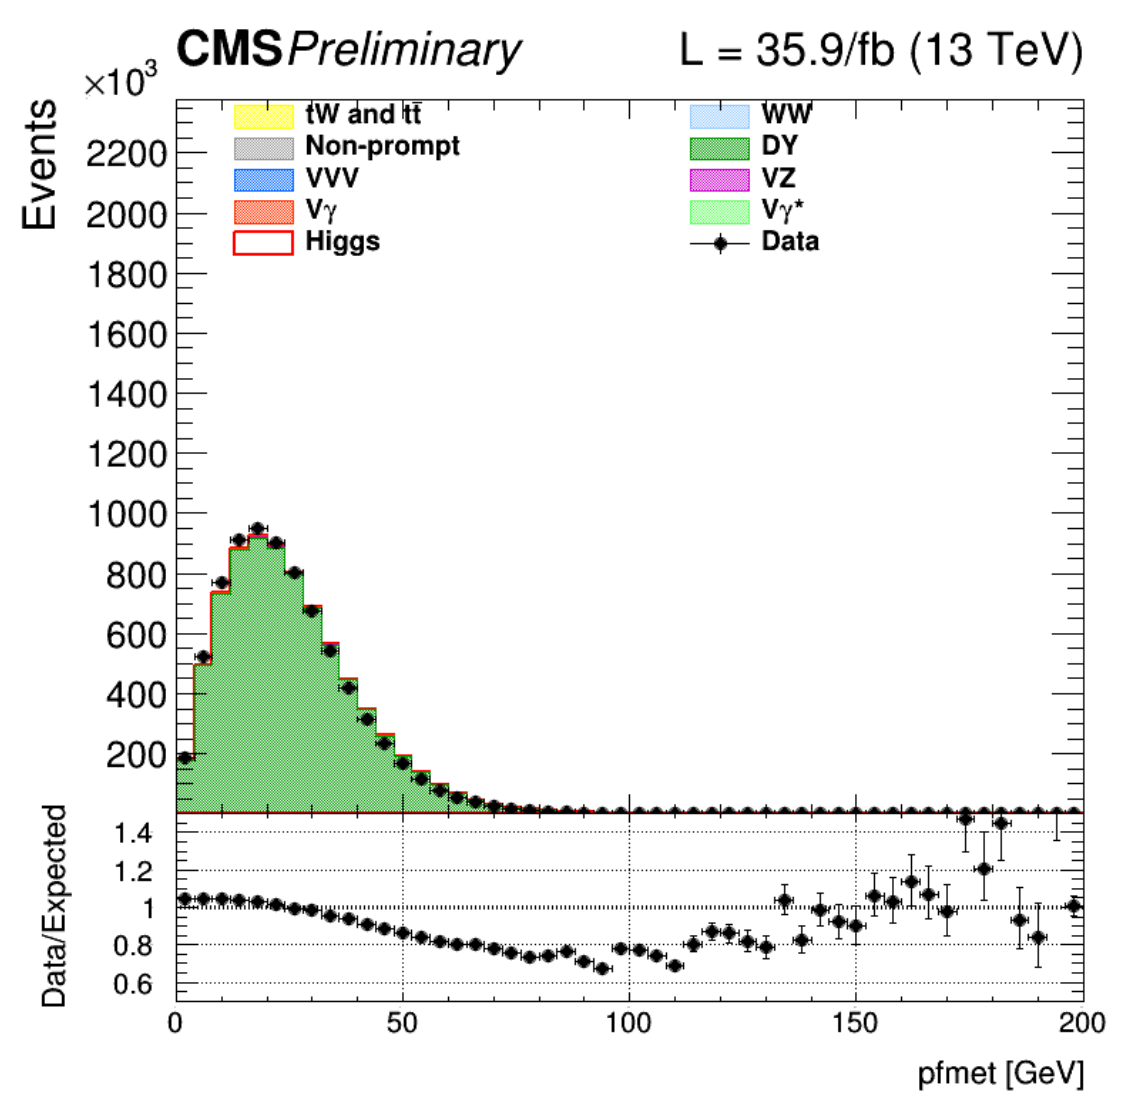
\includegraphics[scale= 1]{../Cap4/met2}
\caption{ The  $E_T^{miss}$ distribution. }
\label{met}
\end{figure}

